\section{Simulations and Results}\label{sec:Results}
All analog simulations are performed in the language of \textit{AIMSpice} in the \textit{AIM-Spice} computer program. All analog simulations are performed in the language \textit{Verilog}, with the editor \textit{VSCode}, compiler \textit{Icarus Verilog} and waveform plotter \textit{gtkwave}.

\subsection{Analog bitcell}
The analog behavior of the bitcell is simulated to show the functionality at different temperatures and with different configurations of slow/fast nmos/pmos transistors, as well as the read-time, the write-time and the leakage current for the SS, TT and FF (TODO?: refer to theory) configurations. TODO: refer to appendix with code

\subsubsection{Leakage current}
The leakage currents at different configurations are shown in \autoref{fig:04:leakage}. The current is negative, so keep in mind that it is the absolute value of the current which is of interest, and is ideally as close to zero as possible.
\begin{figure}[H]
    \centering
    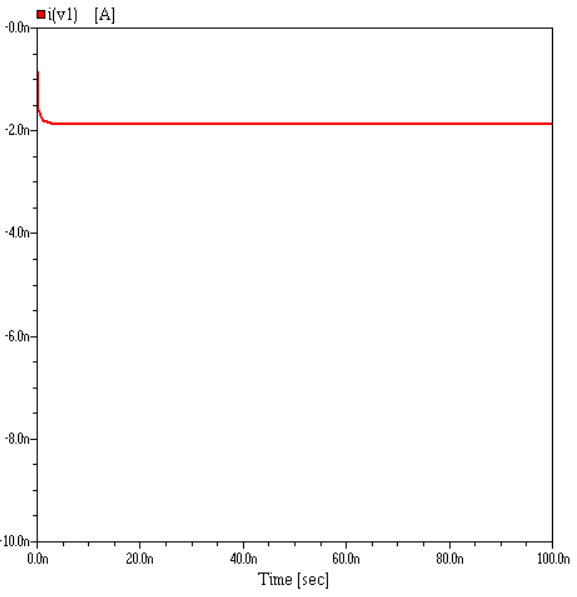
\includegraphics[width=0.3\linewidth]{aimSpice/plots/plotsSS/leak.png}
    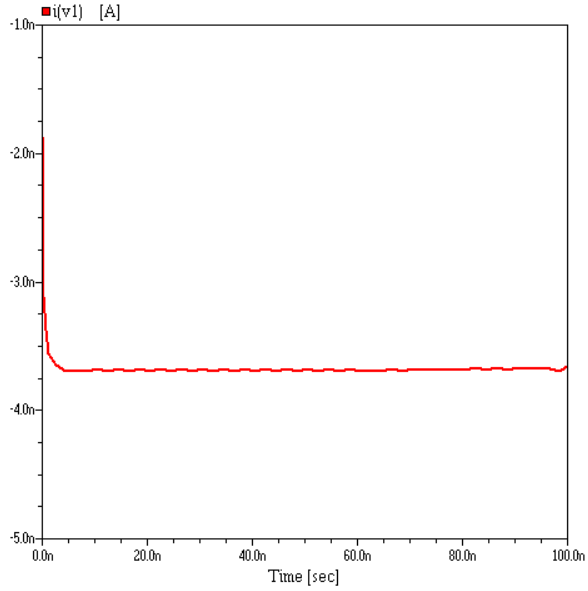
\includegraphics[width=0.3\linewidth]{aimSpice/plots/plotsTT/leak.png}
    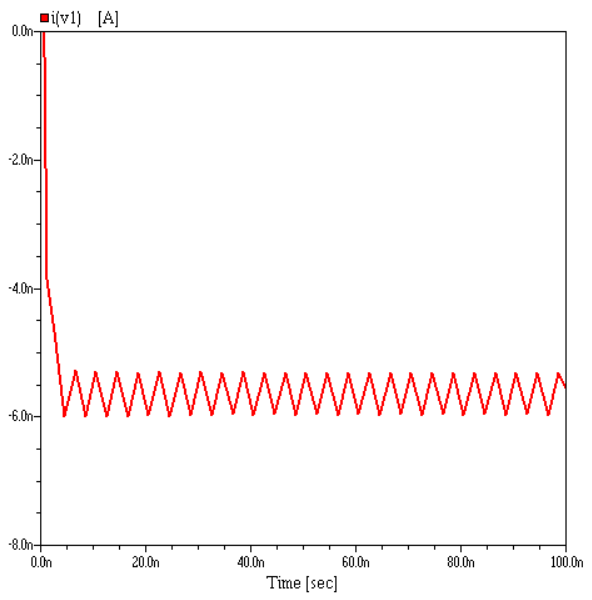
\includegraphics[width=0.3\linewidth]{aimSpice/plots/plotsFF/leak.png}
    \caption{Leakage currents at SS, TT and FF (from left to right).}
    \label{fig:04:leakage}
\end{figure}

\subsubsection{Read time}
The read times can be seen in \autoref{fig:04:read}. They are all shorter than 3ns, as was required in the project description.
\begin{figure}[H]
    \centering
    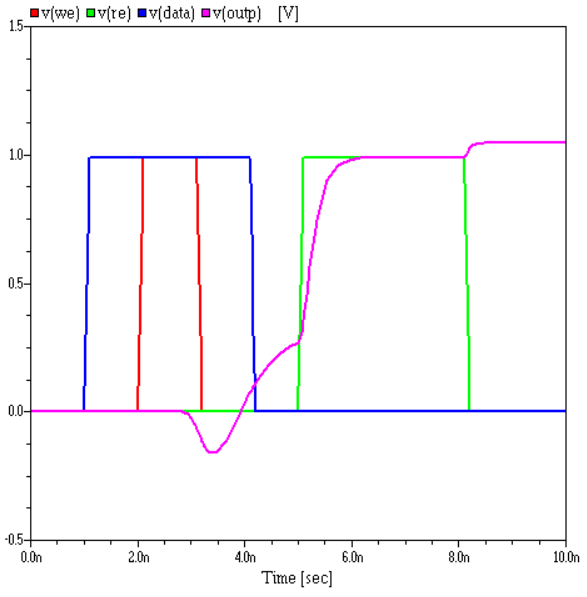
\includegraphics[width=0.3\linewidth]{aimSpice/plots/plotsSS/read.png}
    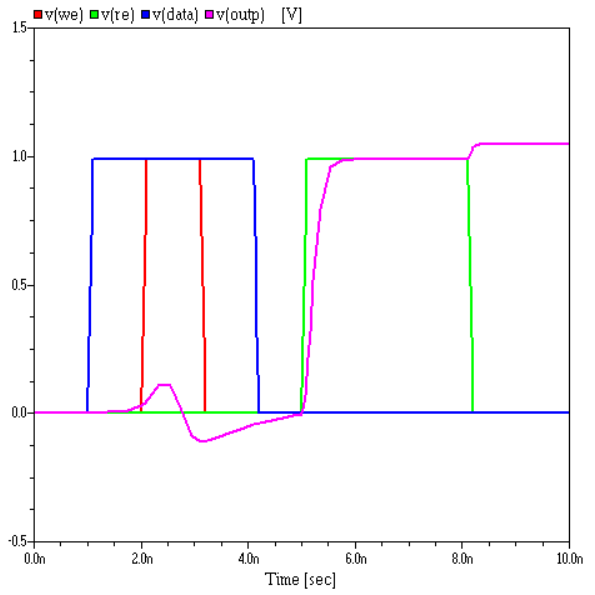
\includegraphics[width=0.3\linewidth]{aimSpice/plots/plotsTT/read.png}
    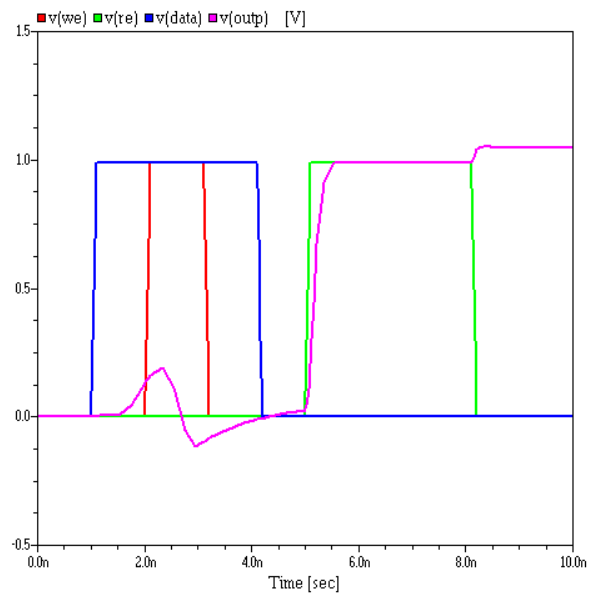
\includegraphics[width=0.3\linewidth]{aimSpice/plots/plotsFF/read.png}
    \caption{The read times to the bitcell at SS, TT and FF (from left to right) can be read as the time it takes v(outp) to reach v(re).}
    \label{fig:04:read}
\end{figure}

\subsubsection{Write time}
The write times can be seen in \autoref{fig:04:read}. They are also all shorter than 3ns, as was required in the project description.
\begin{figure}[H]
    \centering
    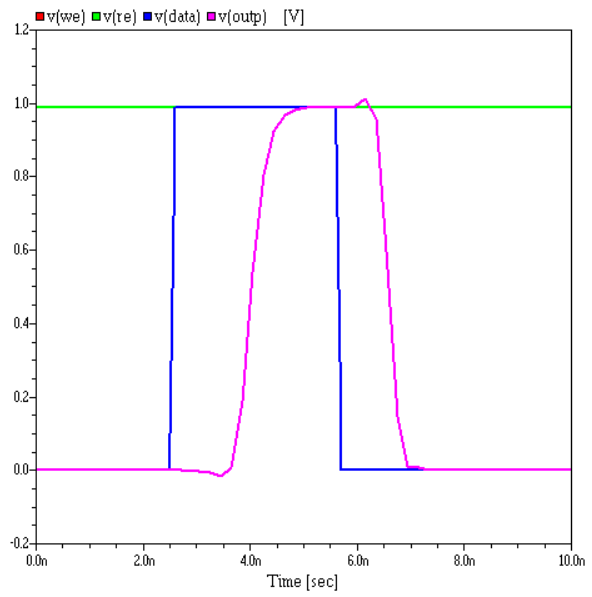
\includegraphics[width=0.3\linewidth]{aimSpice/plots/plotsSS/write.png}
    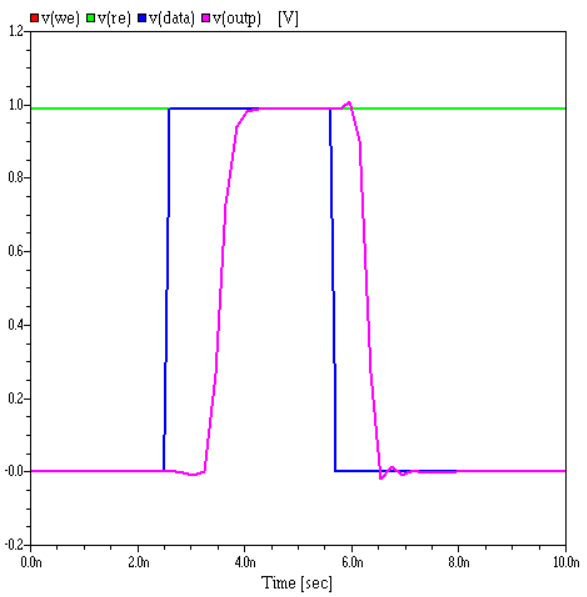
\includegraphics[width=0.3\linewidth]{aimSpice/plots/plotsTT/write.png}
    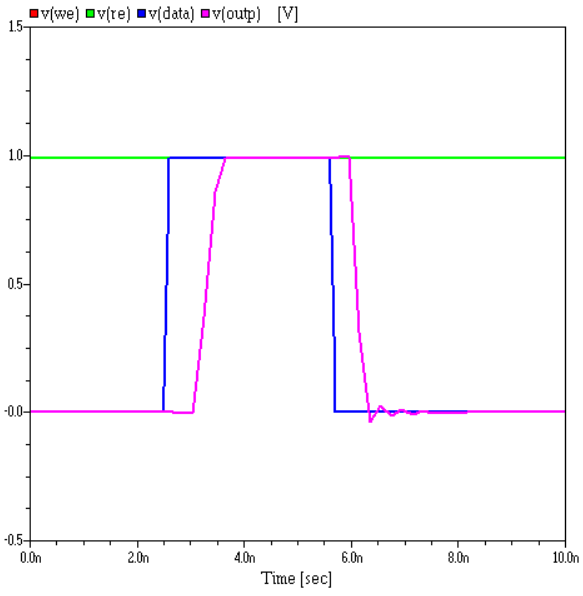
\includegraphics[width=0.3\linewidth]{aimSpice/plots/plotsFF/write.png}
    \caption{The write times to the bitcell at SS, TT and FF (from left to right) can be read as the time it takes v(outp) to reach v(data).}
    \label{fig:04:write}
\end{figure}

\subsubsection{Temperature Functionality}
The circuit is tested at three different temperatures (-20C, 27C, 50C) for five different circuit configurations (FF, FS, SF, SS, TT). The functionality tests all behave as desired, and can be seen in \autoref{fig:04:func}. The test is comprised of writing and reading both low and high to the bitcell. 

\begin{figure}[H]
    \centering
    FF:
    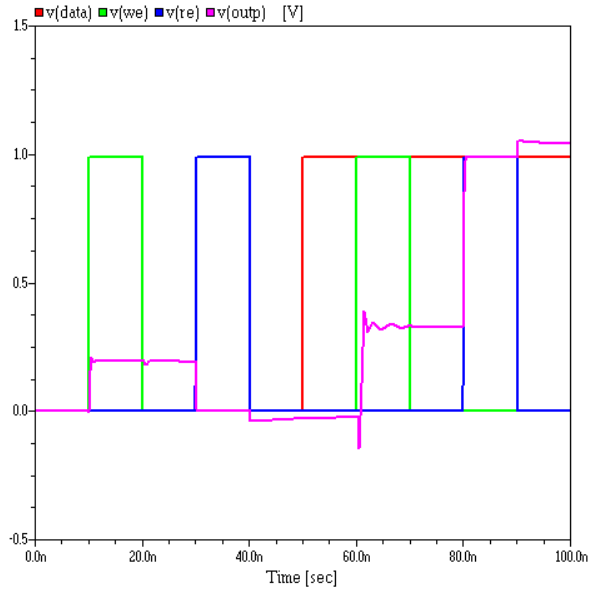
\includegraphics[width=0.24\linewidth]{aimSpice/plots/plotsFF/func-20c.png}
    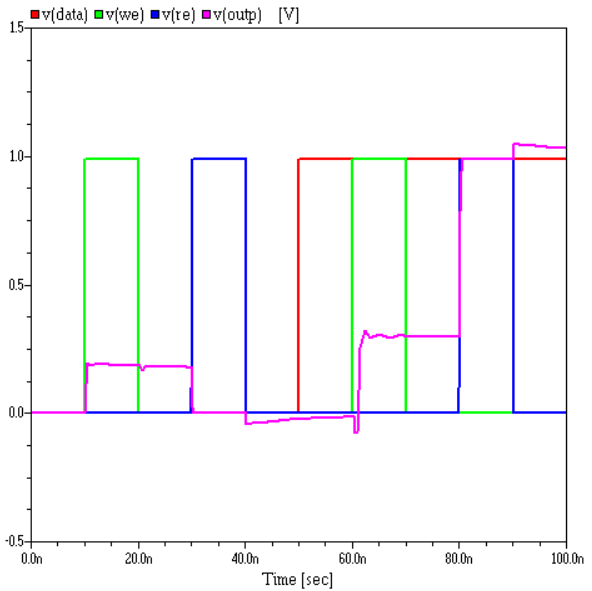
\includegraphics[width=0.24\linewidth]{aimSpice/plots/plotsFF/func27c.png}
    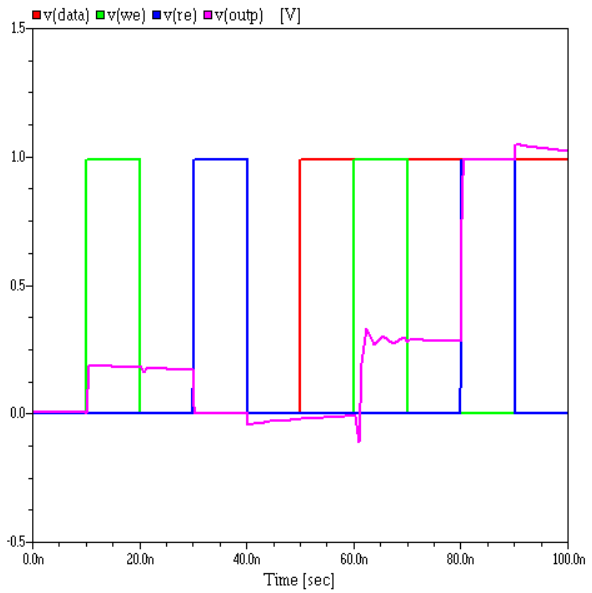
\includegraphics[width=0.24\linewidth]{aimSpice/plots/plotsFF/func50c.png}
    \newline
    FS:
    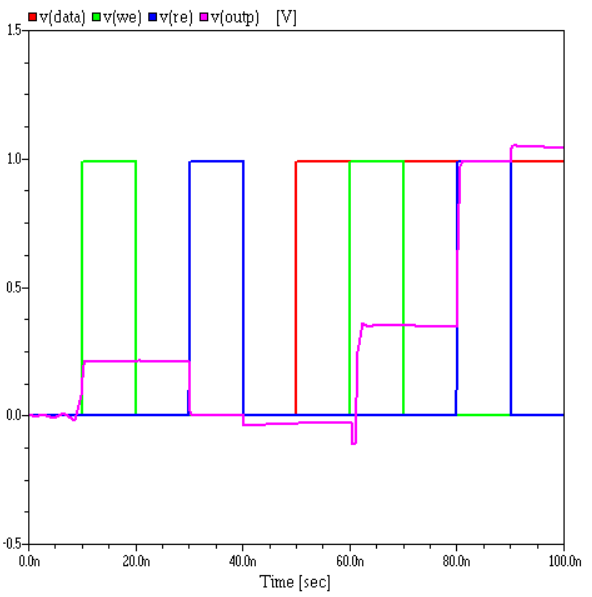
\includegraphics[width=0.24\linewidth]{aimSpice/plots/plotsFS/func-20c.png}
    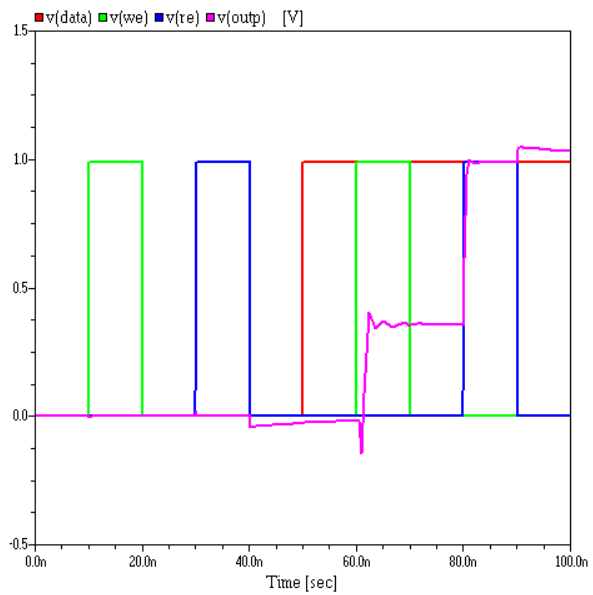
\includegraphics[width=0.24\linewidth]{aimSpice/plots/plotsFS/func27c.png}
    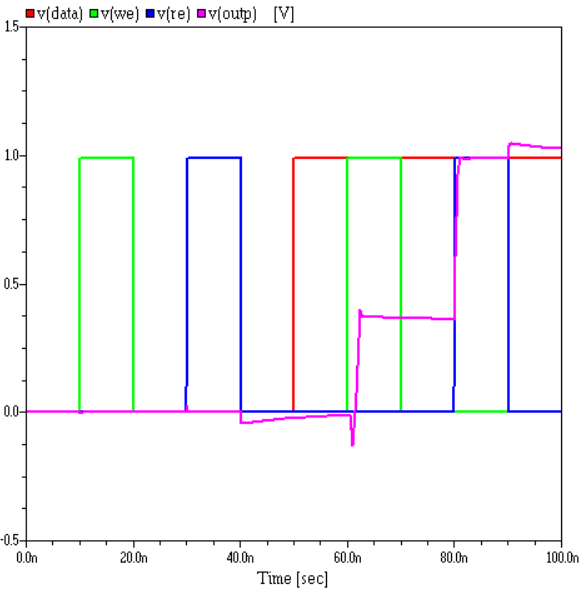
\includegraphics[width=0.24\linewidth]{aimSpice/plots/plotsFS/func50c.png}
    \newline
    SF:
    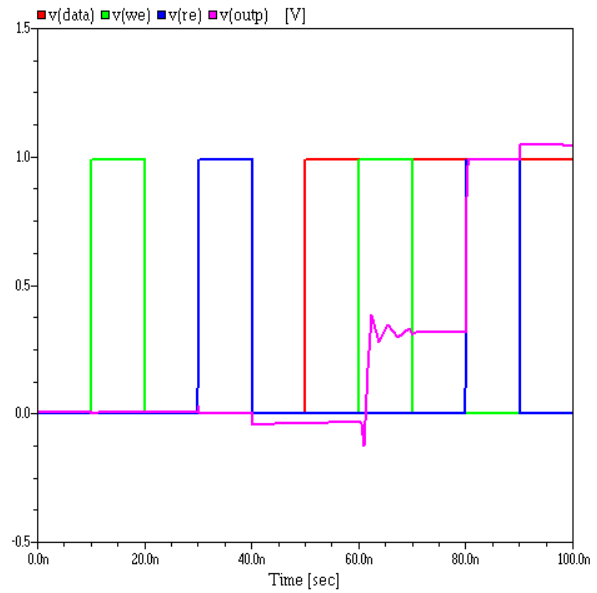
\includegraphics[width=0.24\linewidth]{aimSpice/plots/plotsSF/func-20c.png}
    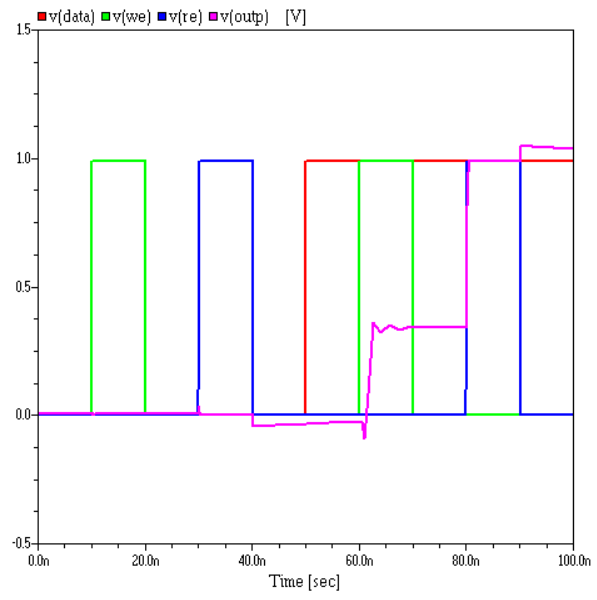
\includegraphics[width=0.24\linewidth]{aimSpice/plots/plotsSF/func27c.png}
    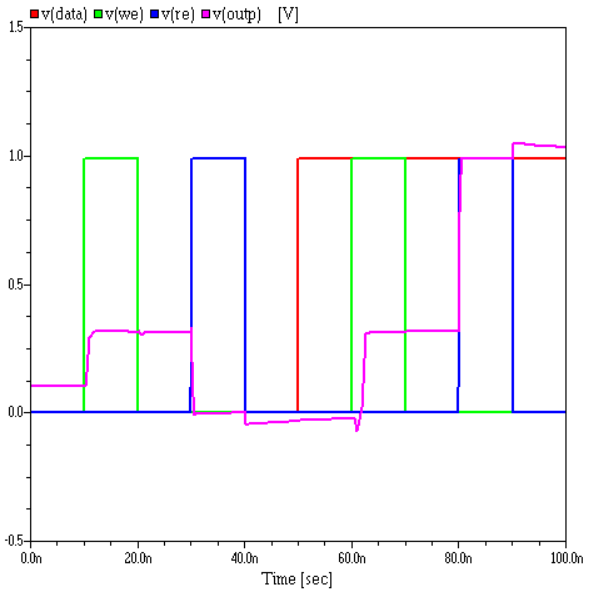
\includegraphics[width=0.24\linewidth]{aimSpice/plots/plotsSF/func50c.png}
    \newline
    SS:
    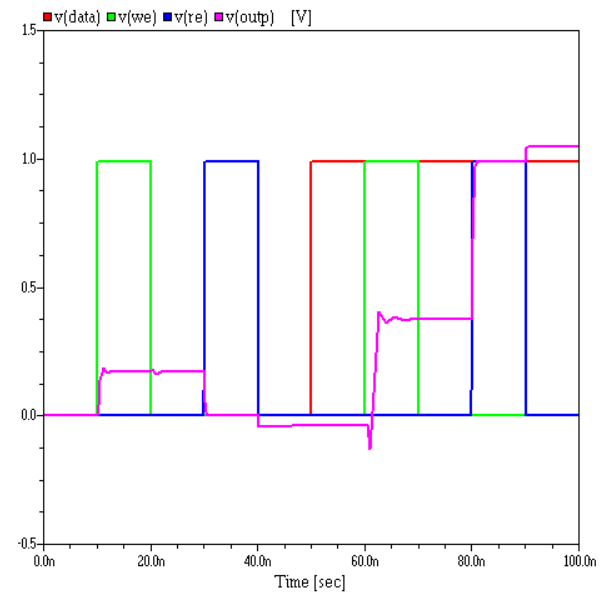
\includegraphics[width=0.24\linewidth]{aimSpice/plots/plotsSS/func-20c.png}
    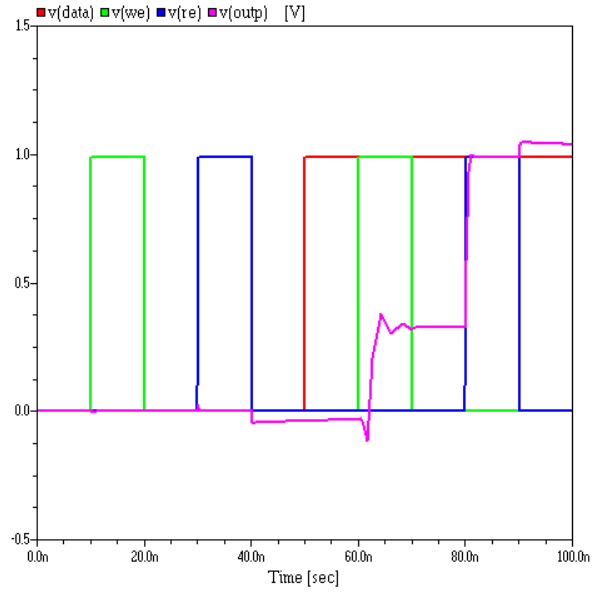
\includegraphics[width=0.24\linewidth]{aimSpice/plots/plotsSS/func27c.png}
    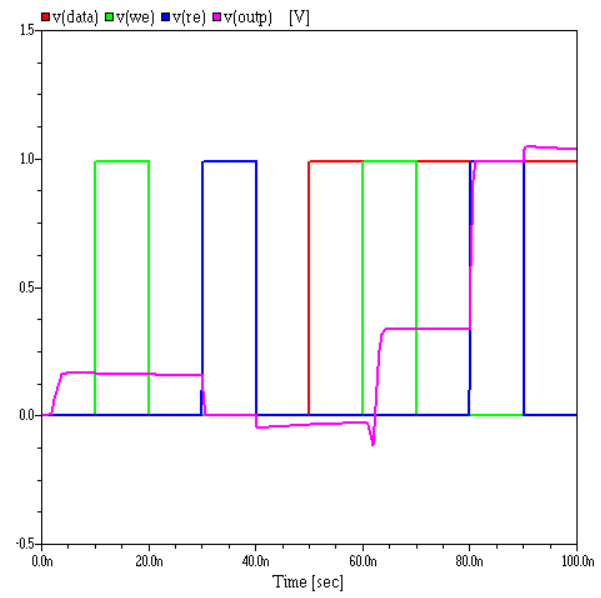
\includegraphics[width=0.24\linewidth]{aimSpice/plots/plotsSS/func50c.png}
    \newline
    TT:
    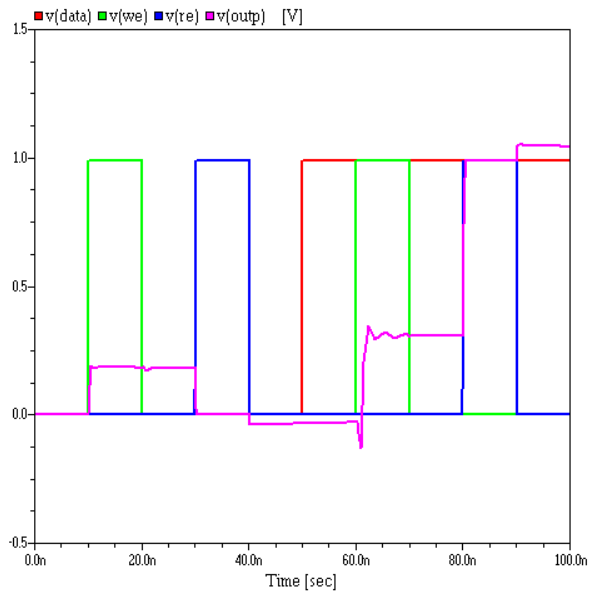
\includegraphics[width=0.24\linewidth]{aimSpice/plots/plotsTT/func-20c.png}
    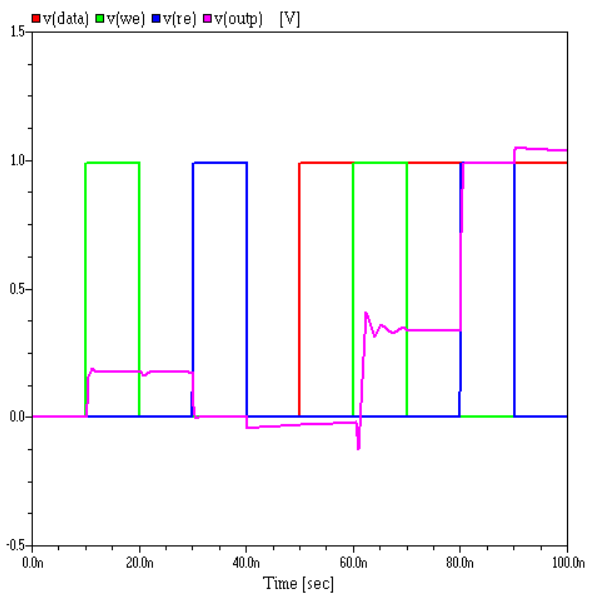
\includegraphics[width=0.24\linewidth]{aimSpice/plots/plotsTT/func27c.png}
    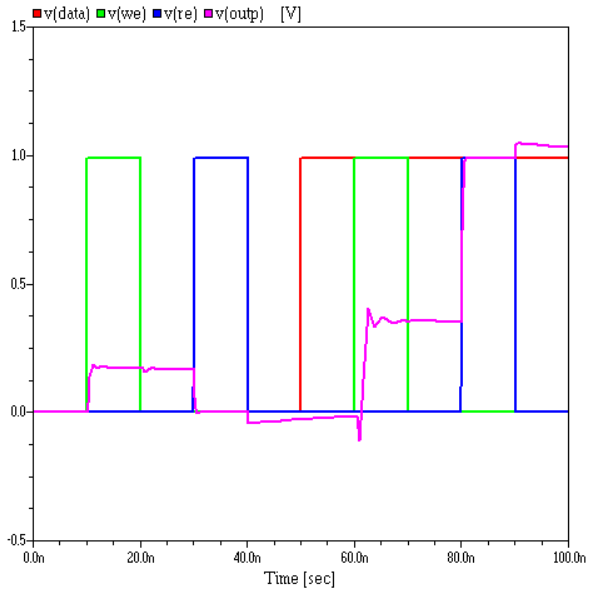
\includegraphics[width=0.24\linewidth]{aimSpice/plots/plotsTT/func50c.png}
    \newline
    
    \caption{The functionality tests of the bitcell. The left column is for -20\degree C, the middle column is for +27\degree C, and the right column is for +50\degree C.}
    \label{fig:04:func}
\end{figure}

\subsection{Digital bitcell}
The bitcell's behaviour is digitally simulated with inputs and outputs according to what can be observed in \autoref{fig:04:bitcell_tb}.

\begin{figure}[H]
    \centering
    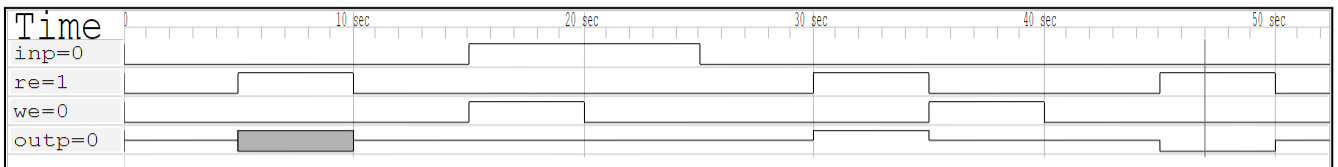
\includegraphics[width=0.9\linewidth]{LaTeX_2/Figures/bitcell_tb.png}
    \caption{Testbench of the bitcell}
    \label{fig:04:bitcell_tb}
\end{figure}

In the testbench we read the bitcell before any value has been set, write a logic high, read the logic high, write a logic low, and read that too. REN is not shown in the figure, since it is trivial.

\subsection{RAM}



\subsection{FSM}



\subsection{Complete memory module}


